\documentclass[a4paper,oneside]{scrarticle}

\usepackage[left=3cm,right=3cm,top=2cm,bottom=2.25cm]{geometry}
\usepackage[ngerman]{babel}
\usepackage{amsmath}
\usepackage{amsfonts}
\usepackage{amssymb}
\usepackage{mathtools}
\usepackage{graphicx}
\usepackage{hyperref}
%\graphicspath{ {./images/} }
\addto\captionsngerman{\renewcommand{\figurename}{Fig.}}


\begin{document}
	\begin{flushleft}
		Bach Nguyen, Johannes Roloff - HTWK Leipzig - INB
	\end{flushleft}
	\begin{center}
		\begin{LARGE}
			\textbf{Muster}
		\end{LARGE}
	\end{center}
	\section*{Station 1}
	Für ein gewähltes Modul eine Sammelmappe erstellen.
	\begin{figure}[h]
		\centering
		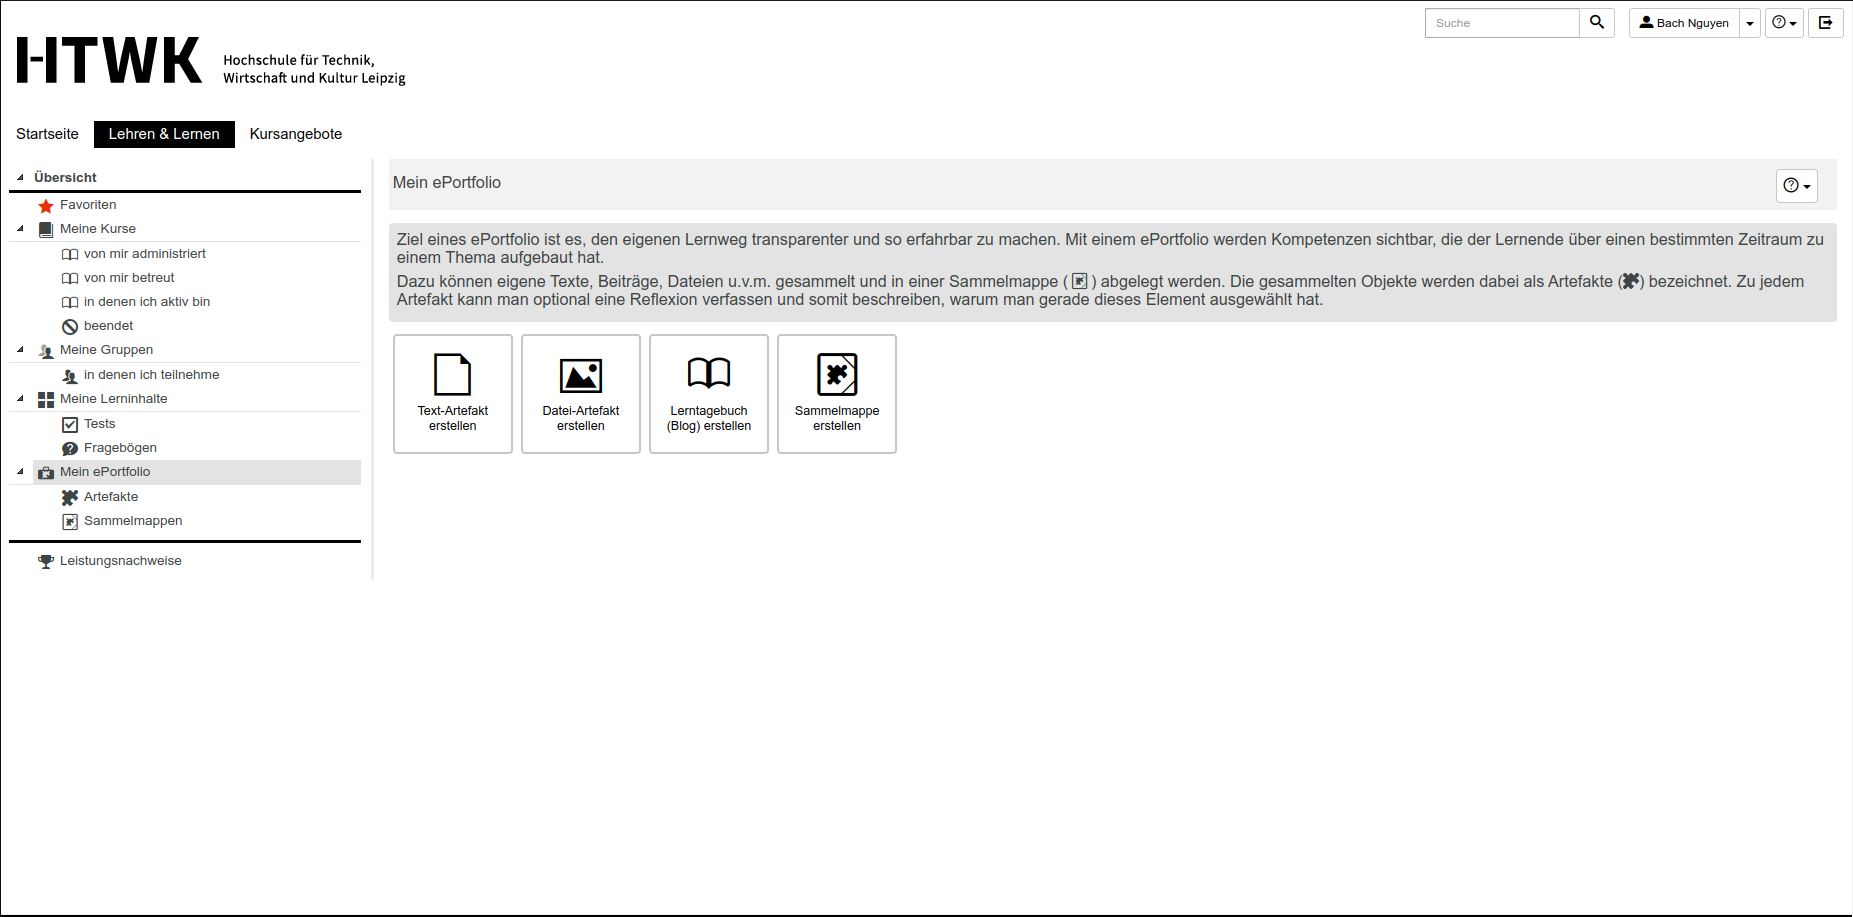
\includegraphics[width=0.8\linewidth]{001_sammelmappeErstellen}
		\caption{Sammelmappe Erstellen}
		\label{fig:001sammelmappeerstellen}
	\end{figure}
	\begin{figure}[h]
		\centering
		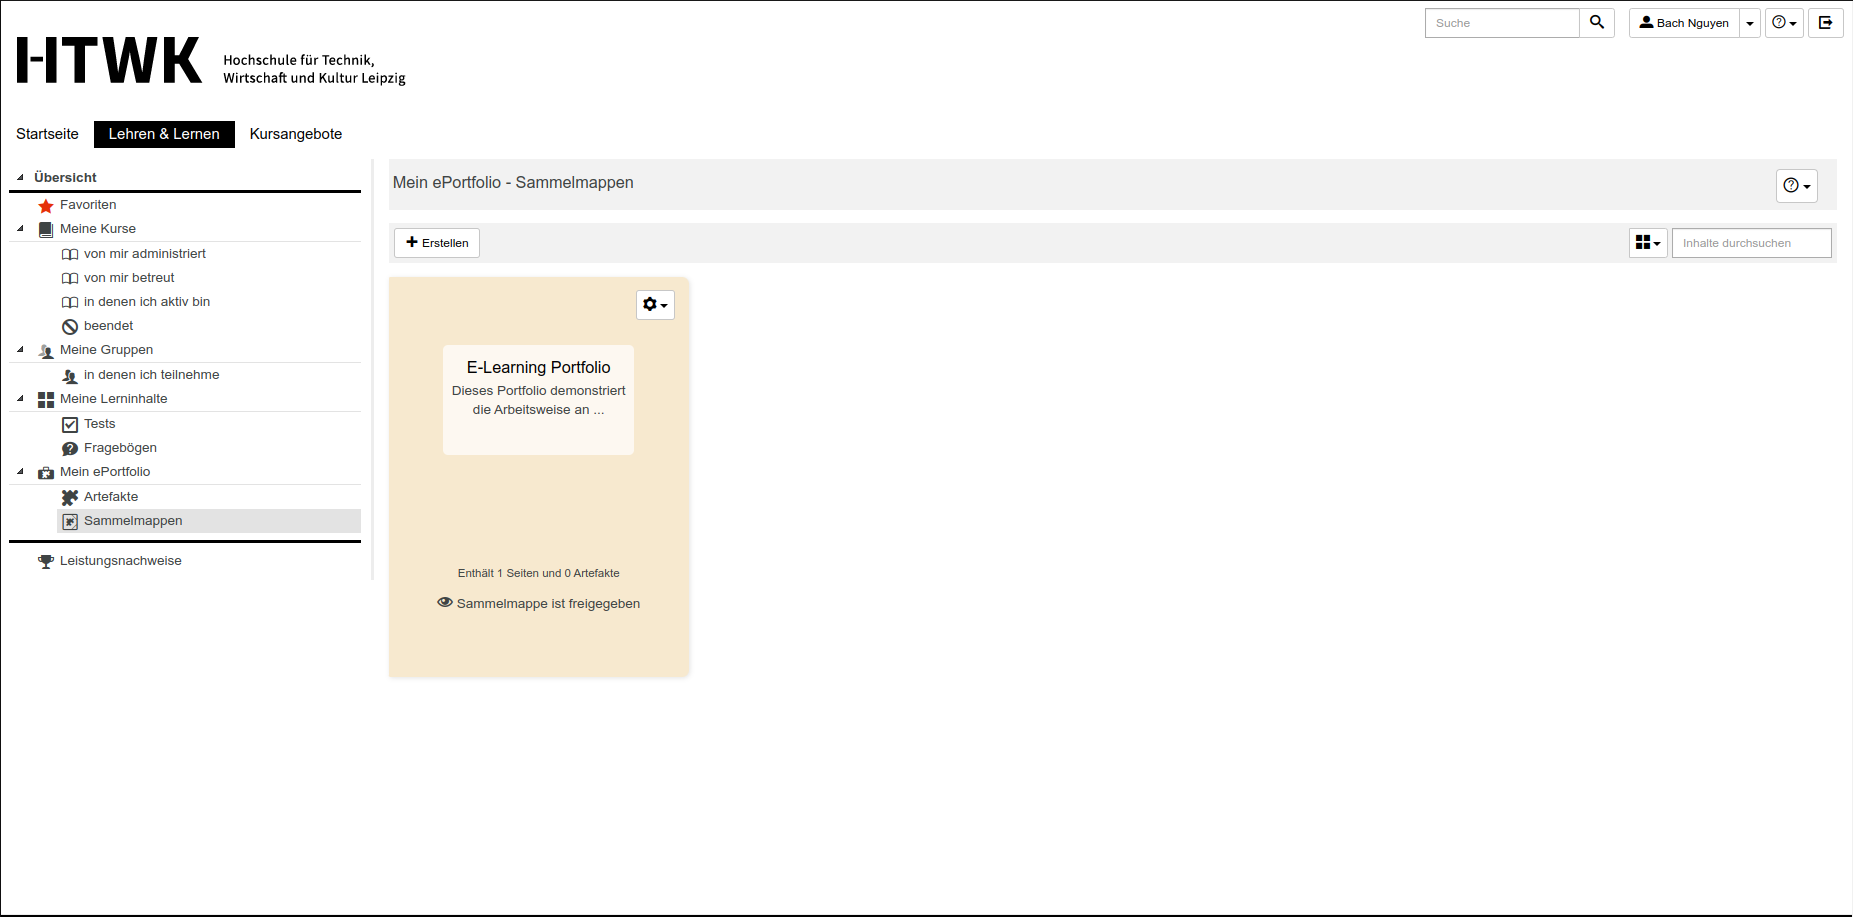
\includegraphics[width=0.8\linewidth]{002_ModulMappe}
		\caption{Modulmappe}
		\label{fig:002modulmappe}
	\end{figure}
	\begin{figure}[h]
		\centering
		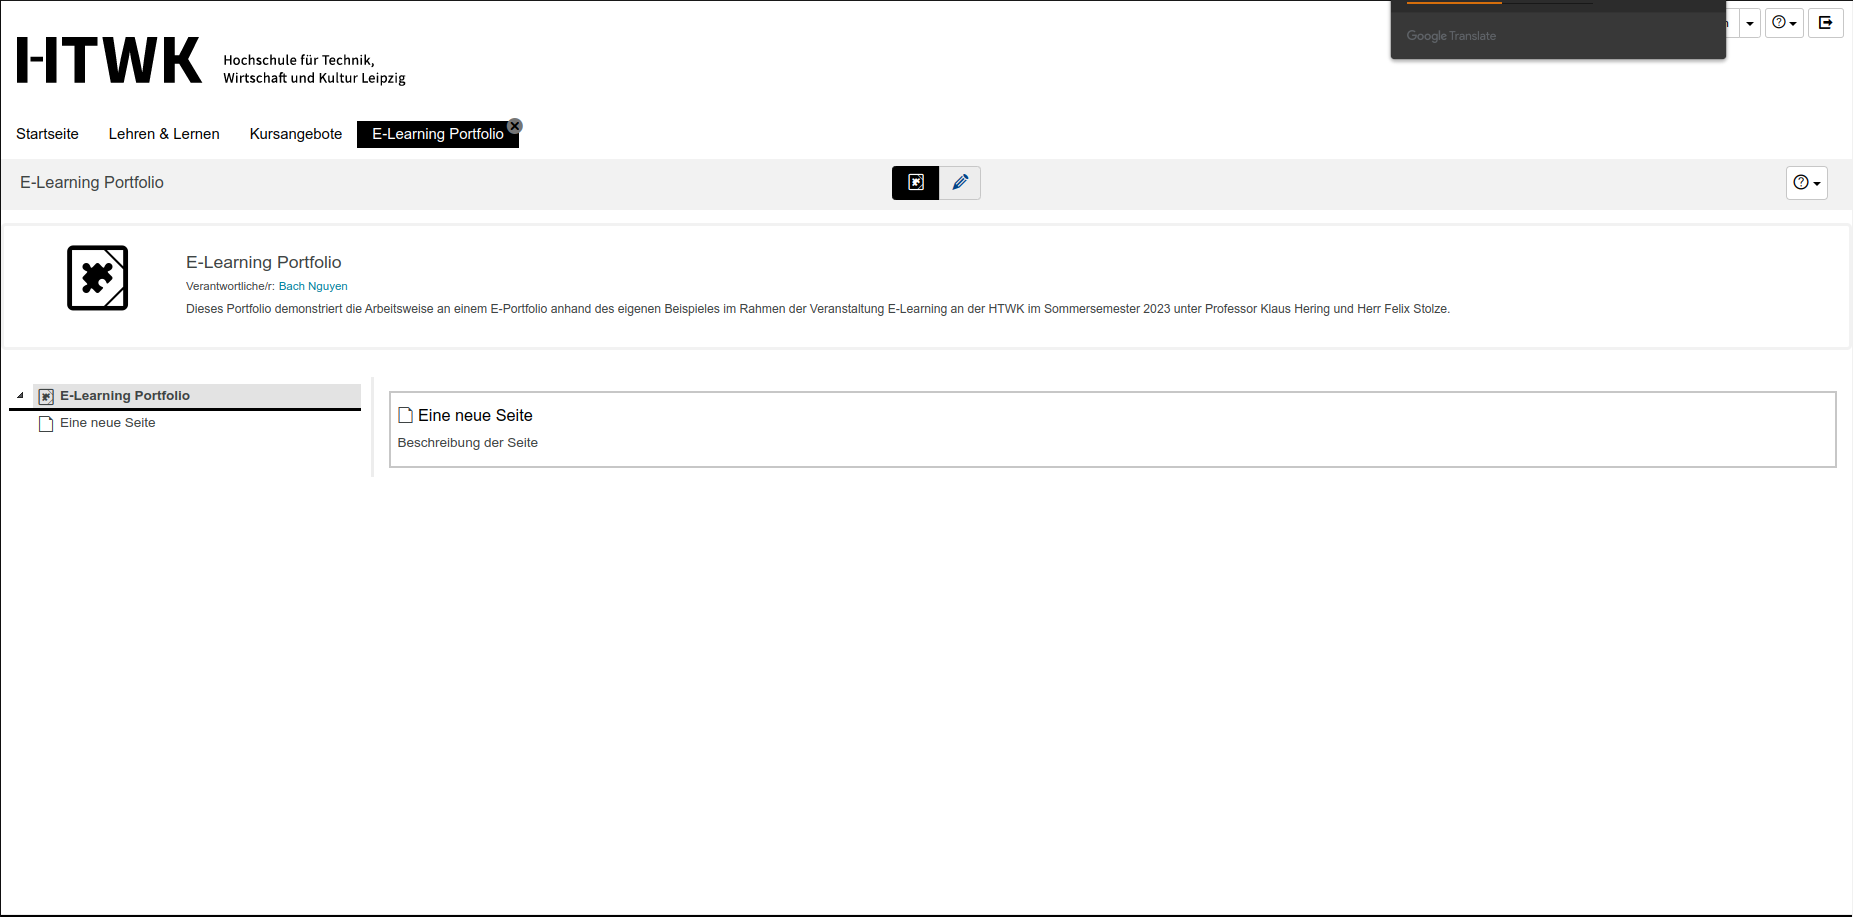
\includegraphics[width=0.8\linewidth]{003_BearbeitungMappe}
		\caption{Mappenbearbeitung}
		\label{fig:003bearbeitungmappe}
	\end{figure}
	\begin{figure}[h]
		\centering
		\includegraphics[width=0.8\linewidth]{"005_beispiel hinzufügen von Artefakten"}
		\caption{Beispiel Hinzufügen von Artefakten}
		\label{fig:005beispiel-hinzufugen-von-artefakten}
	\end{figure}
	\begin{figure}[h]
		\centering
		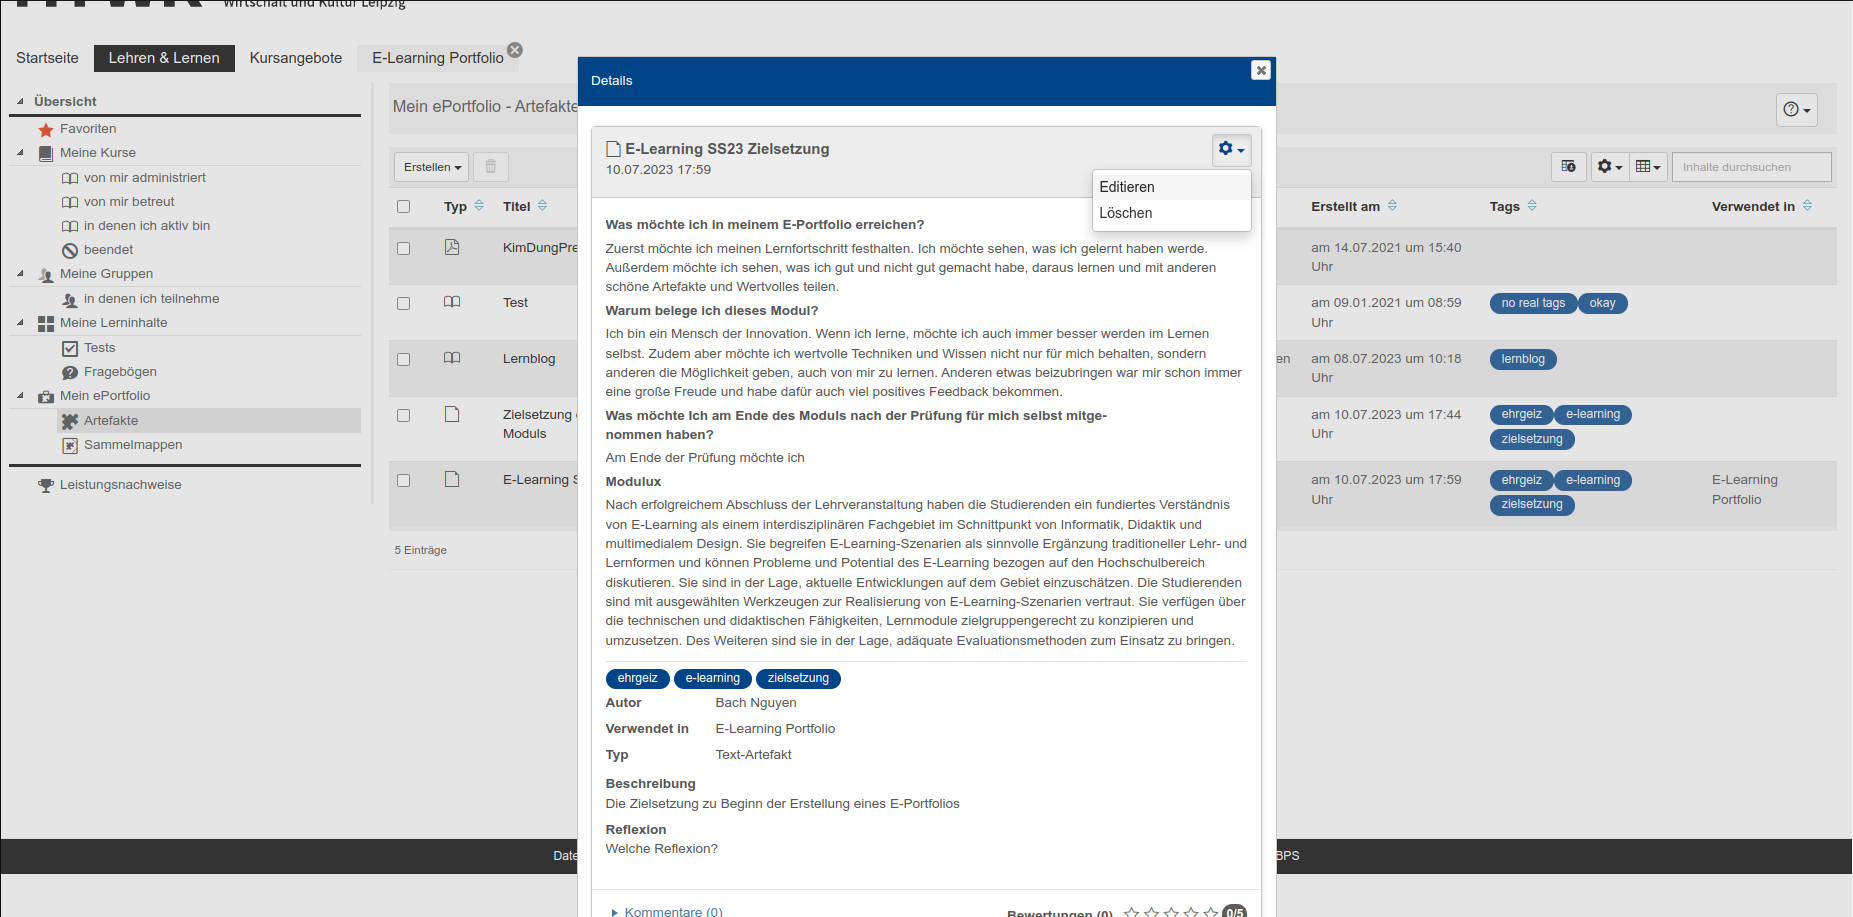
\includegraphics[width=0.8\linewidth]{006_ArtefakteEditieren}
		\caption{Artefakte Editieren}
		\label{fig:006artefakteeditieren}
	\end{figure}\\
	Leider werden PDF Dateien noch nicht mit einer Vorschau/direkten Anzeige unterstützt.\\
	\begin{figure}[h]
		\centering
		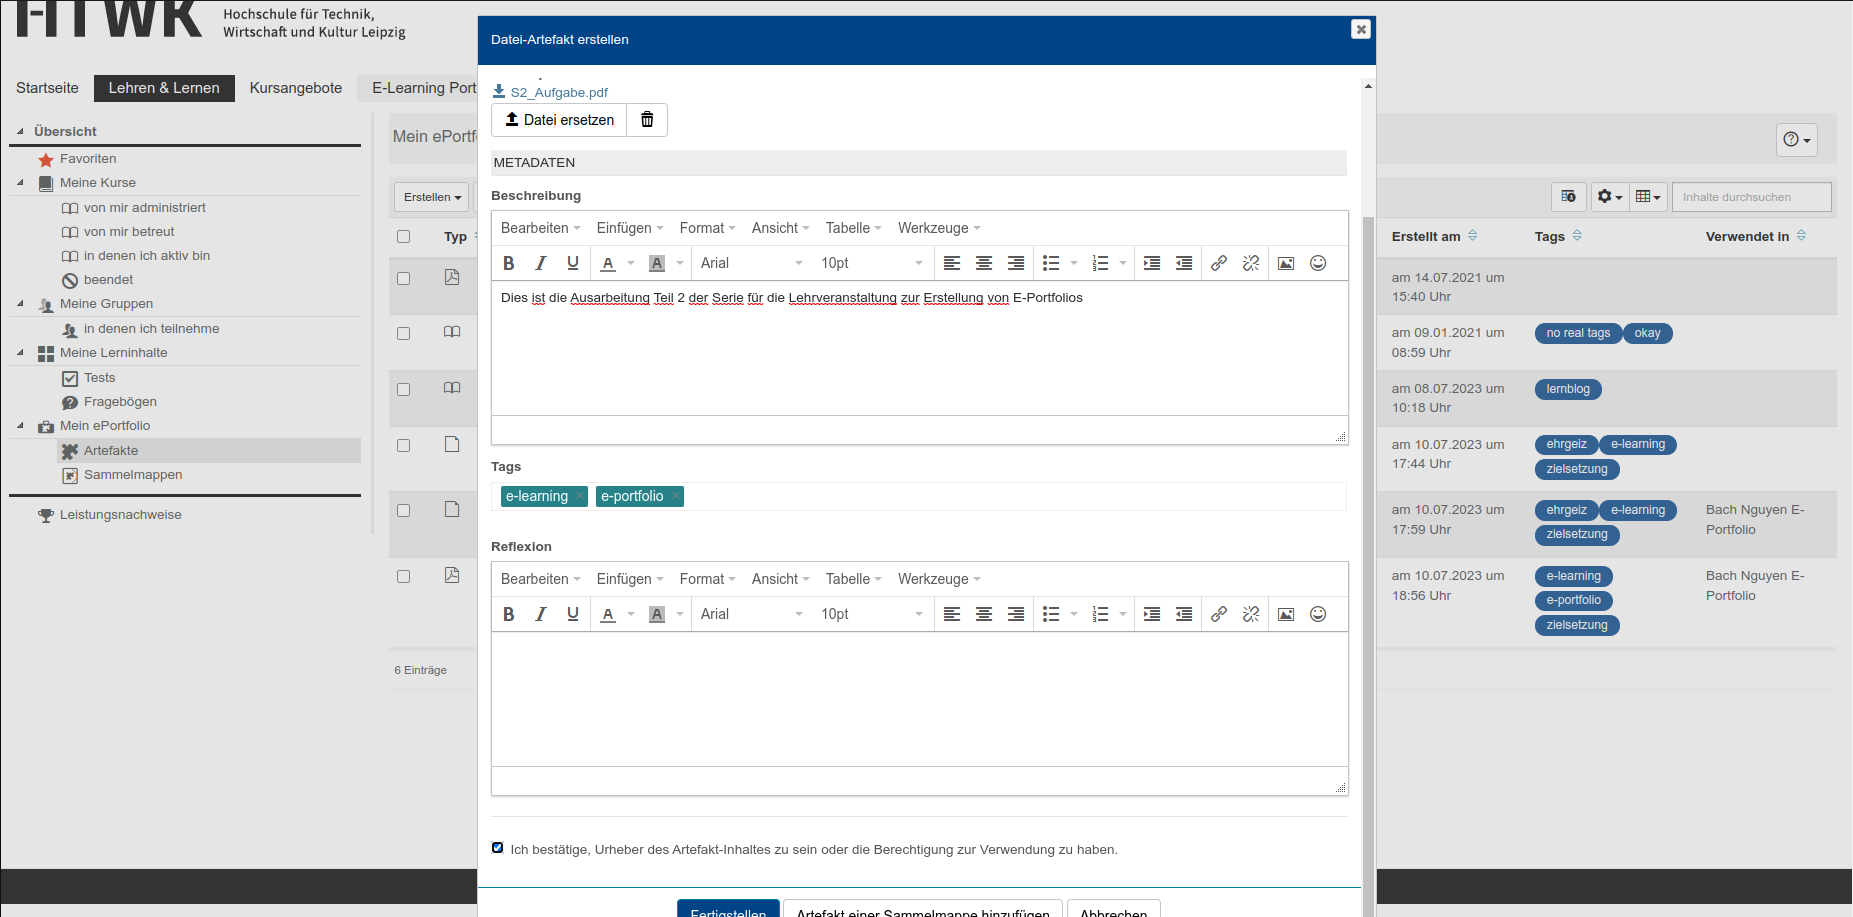
\includegraphics[width=0.8\linewidth]{007_ArtefakteHinzufugen}
		\caption{Datei als PDF hochladen}
		\label{fig:007artefaktehinzufugen}
	\end{figure}\\
\pagebreak
	\href{https://bildungsportal.sachsen.de/opal/auth/MapInvitation/1688783325130451012?4}{Beispiel E-Portfolio}
	\begin{figure}[h]
		\centering
		\includegraphics[width=0.8\linewidth]{"009_beispiel vom endportfolio"}
		\caption{Portfolio Beispiel}
		\label{fig:009beispiel-vom-endportfolio}
	\end{figure}
	\begin{figure}[h]
		\centering
		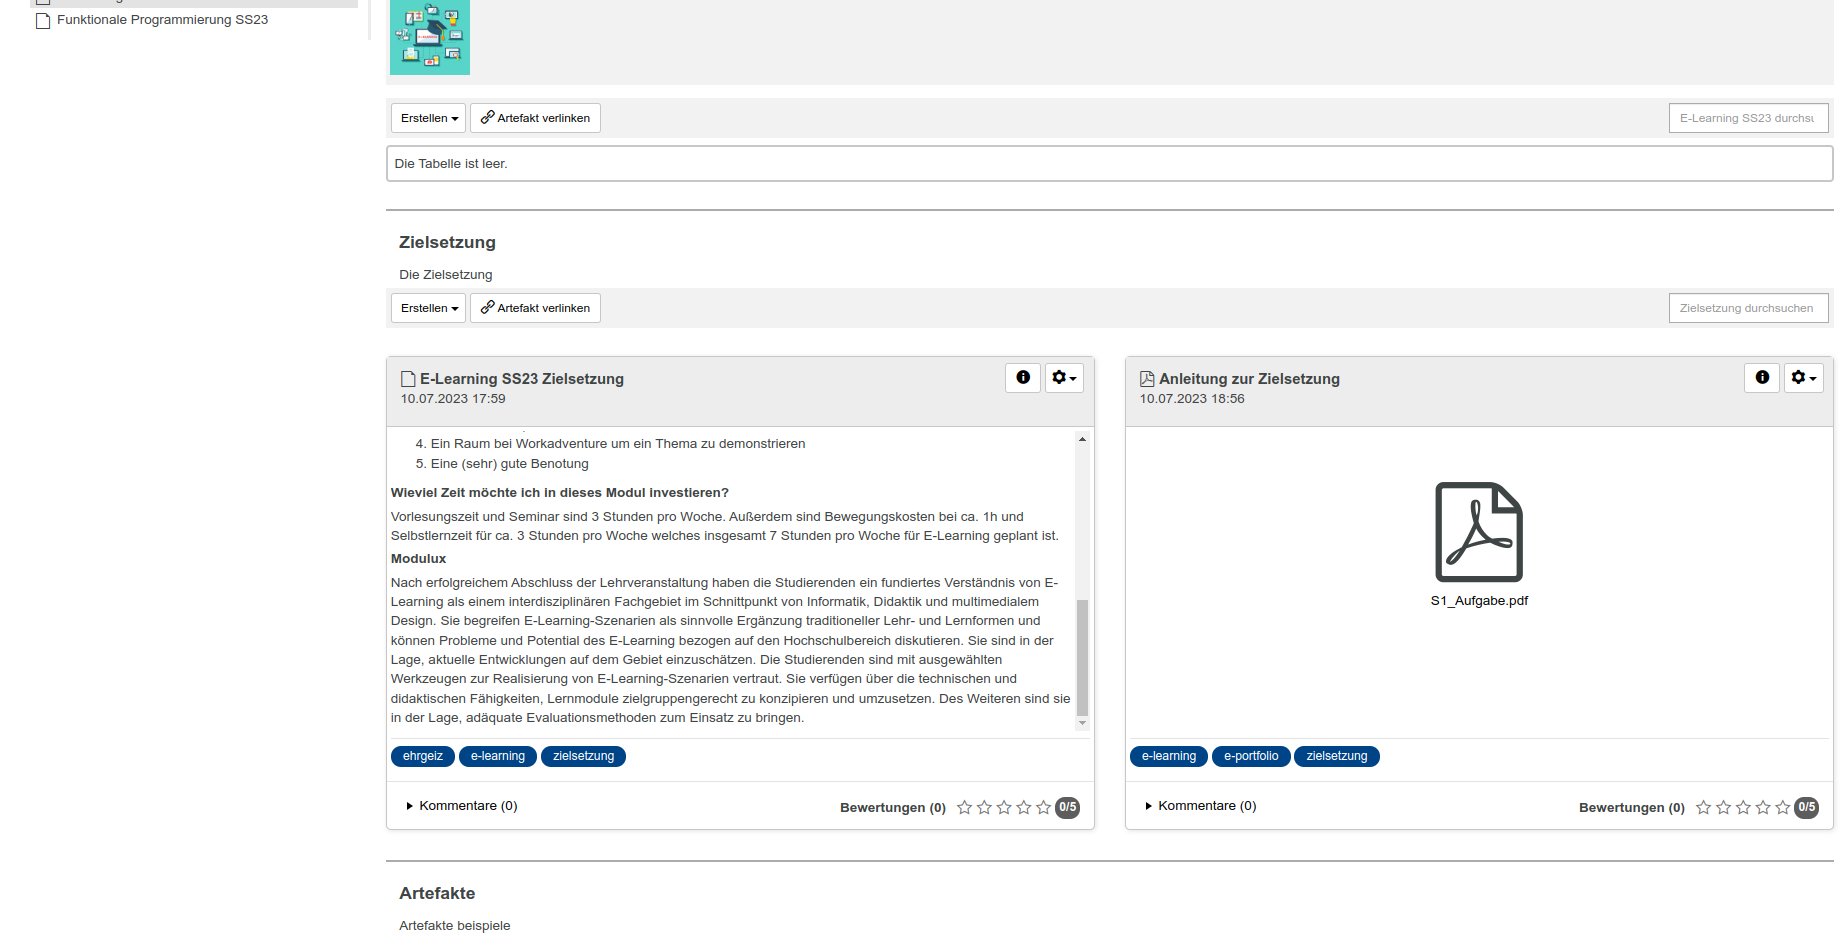
\includegraphics[width=0.8\linewidth]{010_beispielPortfolio2}
		\caption{Beispiel Portfolio E-Learning}
		\label{fig:010beispielportfolio2}
	\end{figure}
	
	
	
	



\end{document}
